\documentclass[aspectratio=43]{beamer}
\usetheme{Berlin}

\title{Sample Title}
\subtitle{Sample Subtitle}
\usepackage[czech]{babel}
\usecolortheme{dolphin}
\usepackage{graphicx}
\usepackage{dirtree}
\usepackage{listings}
\usepackage[utf8]{inputenc}
\usepackage{caption}		% popisky

\captionsetup{labelformat=empty}

\defbeamertemplate*{title page}{customized}[1][]
{
  \usebeamerfont{title}\inserttitle\par
  \usebeamerfont{subtitle}\usebeamercolor[fg]{subtitle}\insertsubtitle\par
  \bigskip
  \usebeamerfont{author}\insertauthor\par
  \usebeamerfont{institute}\insertinstitute\par
  \usebeamerfont{date}\insertdate\par
  \usebeamercolor[fg]{titlegraphic}\inserttitlegraphic
}

\hypersetup{unicode}
\hypersetup{breaklinks=true}

\usepackage{color}
\definecolor{pblue}{rgb}{0.13,0.13,1}
\definecolor{pgreen}{rgb}{0,0.5,0}
\definecolor{pred}{rgb}{0.9,0,0}
\definecolor{pgrey}{rgb}{0.46,0.45,0.48}


\lstset{language=Java,
  showspaces=false,
  showtabs=false,
  tabsize=4,
  breaklines=true,
  showstringspaces=false,
  breakatwhitespace=true,
  commentstyle=\color{pgreen},
  keywordstyle=\color{pblue},
  stringstyle=\color{pred},
  basicstyle=\ttfamily,
  moredelim=[il][\textcolor{pgrey}]{$$},
  moredelim=[is][\textcolor{pgrey}]{\%\%}{\%\%},
}


\title{GraphDraw}
\subtitle{Ročníková práce}
\author{Havránek Kryštof 1.E}
\date{\today}
\institute{Gymnázium, Praha 6, Arabská 14}
\setbeamertemplate{sidebar right}{}
\setbeamertemplate{footline}{%
\hfill\textbf{\insertframenumber{}/\inserttotalframenumber}}


\begin{document}
	\begin{frame}[plain]
		\maketitle
	\end{frame}
	\frame{
		\frametitle{Úvod}
		\section{Úvod}
	\begin{itemize}
		\item Uživatelsky přívětivou aplikaci pro zobrazování grafů matematických funkcí
		\item Zdrojový kód na GitHubu pod licencí WTFPL
		\item Cíle práce
			\begin{itemize}
			\item Schopnost zobrazit grafy
			\item Možnost přiblížení a další operace
			\item Export a import z/do JSON
			\item Později: hledání průsečíků
		\end{itemize}
	\end{itemize}

	}
	\frame{
		\frametitle{Technologie}
		\section{Technologie}
		\begin{itemize}
			\item Java + knihovna JavaFX
			\item Knihovna JSON
			\item IDE - NetBeans
			\item VCS - GitHub
		\end{itemize}
	}
	\frame{
		\frametitle{Uživatelské prostředí a ovládání -- hlavní scéna}
		\section{Uživatelské prostředí a ovládání}
		\centering
			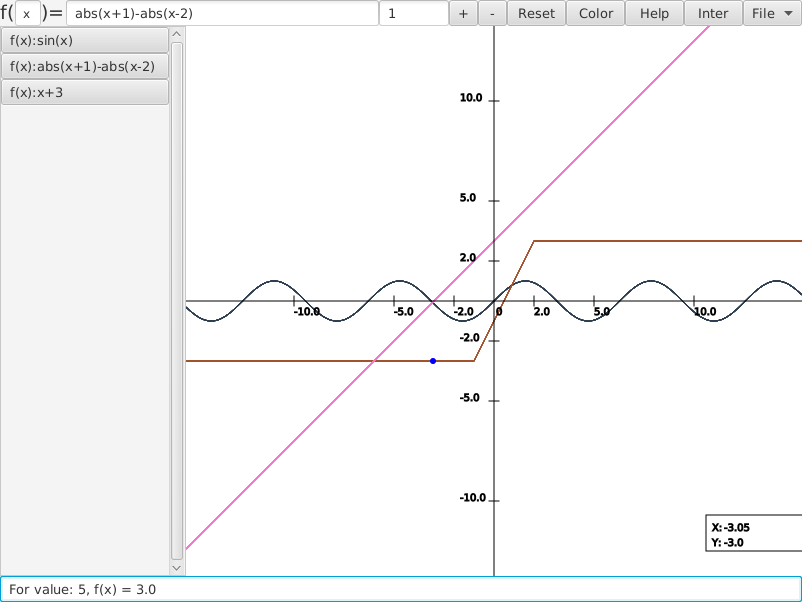
\includegraphics[height=6.9cm]{2019-05-25-152401_802x602_scrot.png}

	}
	\frame{
		\frametitle{Uživatelské prostředí a ovládání -- mód průsečíků}
		\centering
			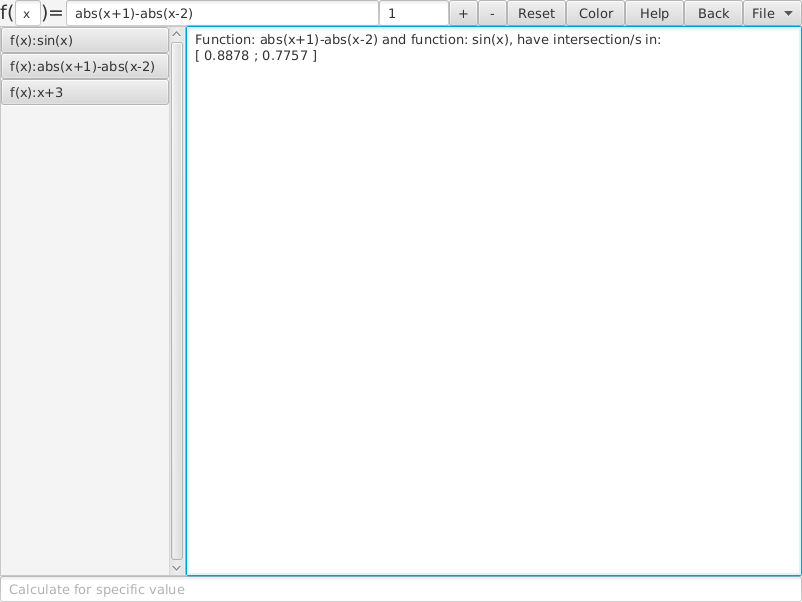
\includegraphics[height=6.9cm]{2019-05-25-152454_802x602_scrot.png}
	}
	\frame{
		\frametitle{Uživatelské prostředí a ovládání -- Ukázka}
		\centering
			Ukázka aplikace
	}

	\frame{
		\frametitle{Backend}
		\section{Backend}
		Struktura souborů
		\dirtree{%
		.1 GraphDraw.
		.2 FXMLDocument.fxml.
		.2 FXMLDocumentController.java.
		.2 GraphGraw.java.
		.2 ParsedExpression.java.
		.2 PosfixExpressionClac.
		.3 OperatorStack.java.
		.3 PostFixExpressionCalc.java.
		.3 Precedence.java.
		}

	}
	\begin{frame}[fragile]
		\frametitle{Backend -- JSON}
\begin{lstlisting}[basicstyle=\tiny,caption={Příklad JSON souboru},captionpos=b]
{
	"functions":[
		{
			"infix":"sin(x)",
			"postfix":"x, sin",
			"color":"#2c3e50",
			"variable":"x"
		},
		{
			"infix":"abs(abs(x+1)-abs(x-2))",
			"postfix":"x, 1, +, abs, x, 2, -, abs, -, abs",
			"color":"#a0522d",
			"variable":"x"
		}
	]
}

\end{lstlisting}

	\end{frame}
	\frame{
		\frametitle{Postfixový kalkulátor}
		\section{Postfix}
		\begin{itemize}
			\item Pro počítače se jedná o superiorní matematický zápis
			\item Jednoduchý výpočet pomocí zásobníku
			\item Převedení do postfixového -- Shunting Yard
			\item Kontrola uživatelova vstupu -- kontrolní výpočty...
			\item Metoda na zjištění Průsečíků dvou funkcí -- Bisection Method
			\item Problém s funkcemi jako je $tan()$
		\end{itemize}
	}
	\frame{
		\frametitle{Postfixový zápis}

		\centering
			\[(6+x)*(x/3)=6, x, +, x, 3, /, *\]
			\[max(sin(x)*3,1.5)=x, sin, 3, *, 1.5, max\]
			\[abs(abs(x+1)-abs(x-2))=x, 1, +, abs, x, 2, -, abs, -, abs\]
	}

	\frame{
		\frametitle{Možná vylepšení}
		\section{Možná vylepšení}
		\begin{itemize}
			\item Metoda na hledání průsečíků je neefektivní
			\item Kontrola uživatelova vstupu
			\item Mód průsečíků zobrazí průsečíky na plátně
			\item Funkce tan a další podobné
			\item GUI $\to$ TUI
		\end{itemize}
	}

\end{document}
